\documentclass{article}

\usepackage{graphicx}
\usepackage{tikz}
\usepackage{tikzsymbols}
\usetikzlibrary{calc,patterns,shapes.geometric}
\pagestyle{empty}
\usepackage[margin=0pt]{geometry}
\geometry{papersize={14in,12in}}

\def\centerarc[#1](#2)(#3:#4:#5){\draw[#1] ($(#2)+({#5*cos(#3)},{#5*sin(#3)})$) arc (#3:#4:#5);}

\begin{document}
	\begin{figure}
		\centering
		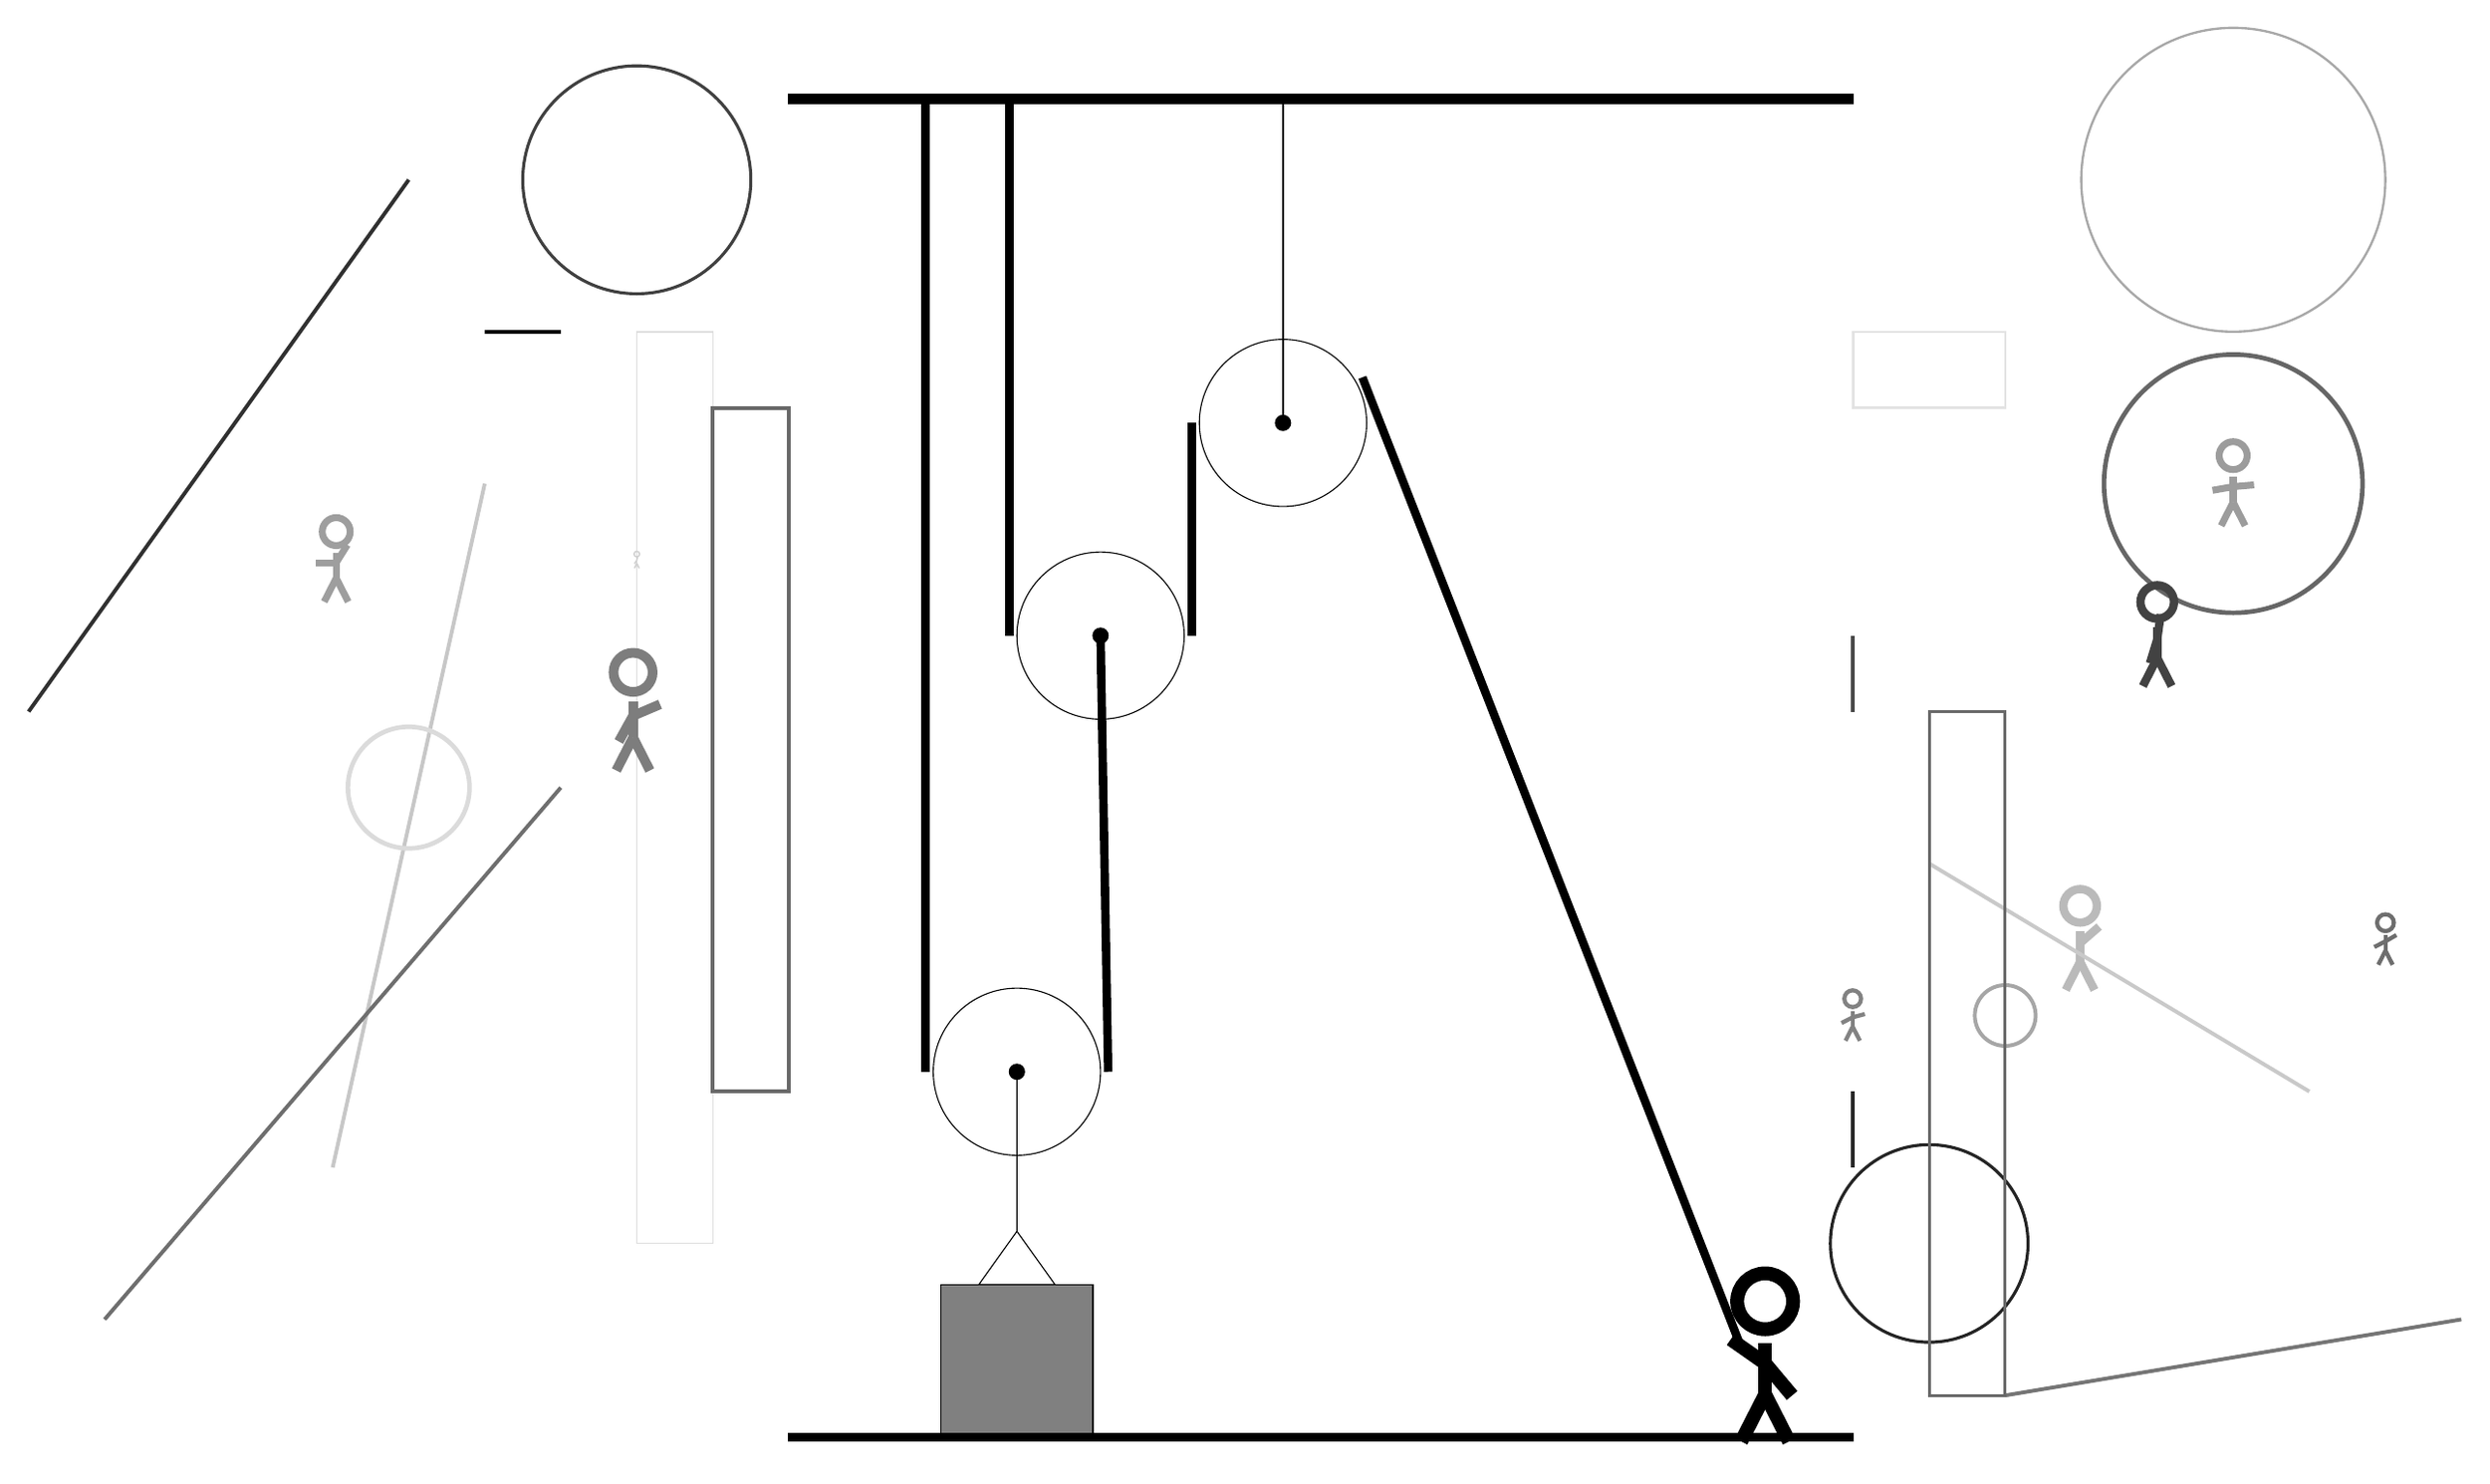
\begin{tikzpicture}
			%%%%% START %%%%%
			
			\draw[fill=black] (-2, 14) rectangle (12, 14.125);
			
			\draw (1, 1.26) circle (1.1);
			\draw[fill=black] (1, 1.26) circle (0.1);
			
			\draw (2.1, 7.0) circle (1.1);
			\draw[fill=black] (2.1, 7.0) circle (0.1);
			
			\node[line width=0.2mm, color=black!38] at (-8, 8) {\Strichmaxerl[5][0][58]};
			
			\draw [line width=0.4mm, color=black!86](13, -1) circle (1.3);
			\draw[line width=0.2mm, color=black!13] (-4, 11) rectangle (-3, -1);
			\draw [line width=0.4mm, color=black!75](-4, 13) circle (1.5);
			\draw [line width=0.3mm, color=black!34](17, 13) circle (2.0);
			\node[line width=0.4mm, color=black!27] at (15, 3) {\Strichmaxerl[6][89][41]};
			
			\draw[line width=0.5mm, color=black!22](-6, 9) -- (-8, 0);
			\node[line width=0.7mm, color=black!49] at (12, 2) {\Strichmaxerl[3][27][15]};
			\draw[line width=0.5mm, color=black!21](13, 4) -- (18, 1);
			\draw[line width=0.5mm, color=black!99](-6, 11) -- (-5, 11);
			\draw[line width=0.5mm, color=black!54](14, -3) -- (20, -2);
			\draw[line width=0.5mm, color=black!81](-7, 13) -- (-12, 6);
			\draw[line width=0.5mm, color=black!59] (-2, 1) rectangle (-3, 10);
			
			\draw [line width=0.6mm, color=black!60](17, 9) circle (1.7);
			\draw [line width=0.5mm, color=black!35](14, 2) circle (0.4);
			\draw[line width=0.3mm, color=black!11] (12, 10) rectangle (14, 11);
			\draw [line width=0.6mm, color=black!14](-7, 5) circle (0.8);
			\draw[line width=0.5mm, color=black!71](12, 6) -- (12, 7);
			\draw[line width=0.5mm, color=black!57](-5, 5) -- (-11, -2);
			
			\node[line width=0.3mm, color=black!51] at (-4, 6) {\Strichmaxerl[7][61][23]};
			\draw[line width=0.5mm, color=black!84] (12, 1) rectangle (12, 0);
			
			\draw[line width=0.4mm, color=black!59] (13, -3) rectangle (14, 6);
			\node[line width=0.3mm, color=black!74] at (16, 7) {\Strichmaxerl[6][73][82]};
			\node[line width=0.6mm, color=black!39] at (17, 9) {\Strichmaxerl[5][10][5]};
			\node[line width=0.7mm, color=black!19] at (-4, 8) {\Strichmaxerl[1][55][78]};
			
			\node[line width=0.4mm, color=black!57] at (19, 3) {\Strichmaxerl[3][27][30]};
			
			\draw (4.5, 9.8) circle (1.1);
			\draw[fill=black] (4.5, 9.8) circle (0.1);
			\draw[thick] (4.5, 9.8) -- (4.5, 14);
			
			\draw (1, 1.26) -- (1, -0.84) -- (0.5, -1.54) -- (1.5, -1.54) -- (1, -0.84);
			\draw[fill=black!50] (0, -1.54) rectangle (2, -3.54);
			
			\draw[line width=1.1mm] (-0.2, 14) -- (-0.2, 1.26);
			\centerarc[line width=1.1mm](1, 1.26)(180:360:1.2000000000000002);
			\draw[line width=1.1mm](2.2, 1.26) -- (2.1, 7.0);
			\draw[line width=1.1mm] (0.9, 14) -- (0.9, 7.0);
			\centerarc[line width=1.1mm](2.1, 7.0)(180:360:1.2000000000000002);
			\draw[line width=1.1mm](3.3, 7.0) -- (3.3, 9.8);
			\centerarc[line width=1.1mm](4.5, 9.8)(30:180:1.2000000000000002);
			\draw[line width=1.1mm] (5.544, 10.4) -- (10.5, -2.3);
			
			\node at (10.8, -2.5) {\Strichmaxerl[10][-35][-50]};
			
			\draw[fill=black] (-2, -3.5) rectangle (12, -3.6);
			
			%%%%% END %%%%%
		\end{tikzpicture}
	\end{figure}	
\end{document}